\begin{refsection}
% DK: I am not sure about the [old] title of this pattern. The bulk of the body of the pattern seems to be about the reuse. Maybe something like “Don’t Make what you can Use” might fit the spirit better. [fixed]


\paragraph{Motivation} This pattern can guide project participants in identifying and managing available resources.

\paragraph{Context}
% DK: This seems like an explanation of the title, not a ``context'' in which a problem is observed.
In a peer production context, you are simultaneously ``making stuff'' and building on the work of others.

\bgroup
\def\arraystretch{1.2}%
\paragraph{Forces}~\hspace{-.04\textwidth}
\begin{tabular}[t]{p{.7\textwidth}@{\hspace{.05\textwidth}}c}
\textbf{Derivative}: you don't have to do everything yourself! & {\icon \symbol{"002159}} \\
\textbf{Sensemaking}: resources are useful only when you can make sense of them. & {\icon \symbol{"00219B}}\\
\textbf{Sharing}: your understanding gains robustness when you share with others. & {\icon \symbol{"00219E}}
\\
\end{tabular}
\egroup


\paragraph{Problem}
Many projects die because the cost of \patternnameext{\href{http://c2.com/cgi/wiki?ReinventingTheWheel}{Reinventing the Wheel}} [c2] is too high.  However, this is just one symptom of overfocus on a few priorities.  Concerns may also arise if the project's output is not actually used by anyone.
%  that it is unable to benefit from connection and relationship. 

\begin{wrapfigure}{l}{.42\textwidth}
\vspace{-.3cm}
{\centering
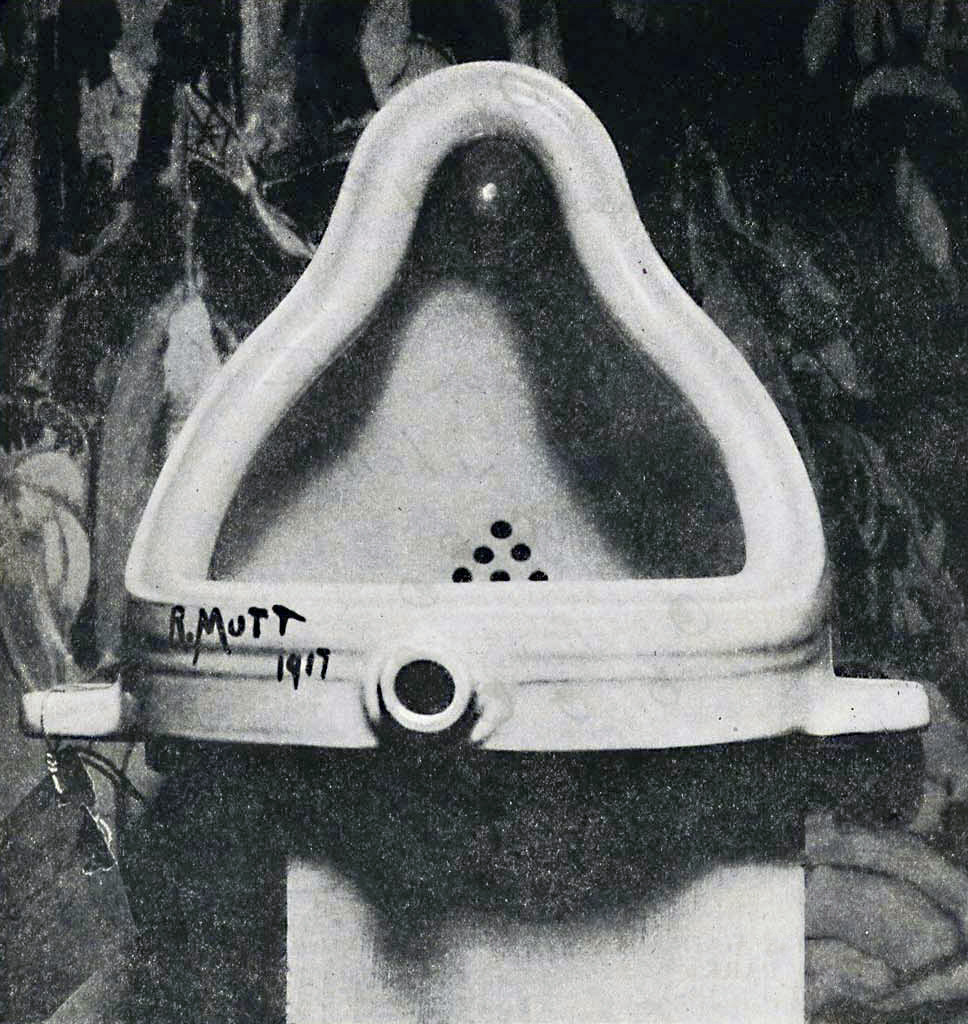
\includegraphics[width=.35\textwidth]{../pictures/Duchamp_Fountaine.jpg}

\par}
\caption{A paradigmatic example of found-art. ``Fountain by R. Mutt, Photograph by Alfred Stieglitz, The exhibit refused by the independents''. 
%Public domain, via the Wikimedia Commons.
\label{fountain}}
\vspace{-1.1cm}
%\vspace{-0.cm}
\end{wrapfigure}


\paragraph{Solution} ``Steal like an artist,'' and make it possible for other people to build on your work too (Figure \ref{fountain}).  In the Peeragogy project, we have used off-the-shelf and hosted software suited to the task at hand (incuding: Drupal, Google+, Google Hangouts, Google Docs, Wordpress, pandoc, Github, ShareLaTeX).  Early on we agreed to release our \emph{Peeragogy Handbook} under the terms of the Creative Commons Public Domain Dedication (CC0), the legal instrument that grants the greatest possible leeway to downstream users.\footnote{\url{https://creativecommons.org/publicdomain/zero/1.0/}}  This has allowed us and others to repurpose and improve its contents in other settings, including our published papers.  Follow the steps indicated by the keywords in the pattern's title: 
\vspace{-1mm}
\begin{itemize}
\item \emph{Reduce} the panoply of interesting interrelated ideas and methods to a functional core (e.g.~writing a book).
\item \emph{Reuse} whatever resources are relevant to this aim, factoring in ``things I was going to have to do anyway'' from everyone involved.
\item  \emph{Recycle} what you've created in new connections and relationships.
\end{itemize}

\paragraph{Rationale} 
Clearly we are not the first people to notice the problems with wheel-reinvention, including ``missing opportunities, repeating common mistakes, and working harder than we need to.''\footnote{\url{https://blog.wikimedia.org/2013/11/19/learning-patterns-new-way-share-important-lessons/}}  As a guest in  one of our hangouts, Willow Brugh, of Geeks without Bounds and the MIT Media Lab, remarked that \emph{people often think that they need to build a community, and so fail to recognize that they are already part of a community.}\footnote{\url{https://www.youtube.com/watch?v=NpyQfYVKfBI}}
We converted our old pattern catalog from the \emph{Peeragogy Handbook} into this paper, sharing it with a new community and gaining new perspectives; could we do something similar again?

\paragraph{Resolution} Reweaving old material into \textbf{derivative} designs and new material into existing frameworks, we build deeper understanding, and carry out collective \textbf{sensemaking}.
%
The project's \patternname{Roadmap} develops by making sense of existing resources -- including our worries and concerns.
Often we only know what these are when we attempt to \textbf{share} them.
Drawing on a wide range of resources boosts our collective \patternname{Carrying capacity}.

%% \paragraph{Inversion}   
%% Novel discoveries may be granted limited monopoly rights, which may make it unprofitable to share them through other than market means.  Use this pattern with care if your aim is to to occupy (or appear to occupy) a monopoly position, or when involving others in your work would have more costs than benefits \cite{coase1937nature}.

\paragraph{Example 1}
Contributors are encouraged to recycle existing works that are compatible
with the Wikimedia-wide CC-By-SA license.
Some subprojects been created purely to help repurpose other existing works in this
way.\footnote{\url{https://en.wikipedia.org/wiki/Wikipedia:WikiProject_Mathematics/PlanetMath_Exchange}}
%
On the downstream side, DBPedia is an important resource for the
semantic web, built by collating data from Wikipedia's
``infoboxes''.\footnote{\url{http://wiki.dbpedia.org/}}
%
These infoboxes are themselves increasingly being populated
automatically using information from WikiData.\footnote{\url{https://www.wikidata.org/wiki/Wikidata:Main_Page}}
Researchers have been able to develop tools that reuse Wikipedia content in other ways \cite{reinhold2006wikitrails,riche2010ichase},
However, these research projects do not always result in a tool that
is accessible to day-to-day users.

\vspace{.05cm}

\paragraph{Example 2}
The knowledge resources and collaboration tools currently available online
are what make a low-cost, high-quality, formally-accredited future university
conceivable.  However, the available resources are not always as
organized as they would need to be for educative purposes, so peeragogues can usefully put
effort into \patternname{Reduce, reuse, recycle}'ing available
resources into a functioning university Library.

%\paragraph{Summary}

\begin{framed}
\noindent 
\emph{What's Next in the Peeragogy Project}
%OSS: Make it less self-referential about paper and project - What other parts of the handbook can we turn into patterns?
\definecollection{ReduceWN}
\begin{collectinmacro}{\ReduceWN}{}{}
Are there other educational resources and peeragogical case studies
that we could fold into our work?  Can we recycle material from the
\emph{Peeragogy Handbook} into a format that is easier to understand
and apply?
\end{collectinmacro}
\ReduceWN
\end{framed}

\printbibliography[heading=subbibliography]
\end{refsection}
